
\chapter{Verification}
\label{sec:verify}

The International Energy Agency has sponsored a number of international
research collaborations to further the state of wind energy technology and
tools.  One of these, Task 30: Offshore Code Comparison Collaboration
(OC3), shared a spar design among many participants to compare
performance as modeled by differed tool sets.  A description of the OC3
spar is provided in \citet{OC3}.  Since it is already a
well-studied geometry, this design was selected as the focus of
verification for \textit{FloatingSE}.  As part of the Task 30 effort,
an ANSYS model of the OC3 spar, using shell elements combined with
stiffeners and bulkheads, was also generated.  This was taken as
the \textit{truth} standard for comparison.

\section{Mass Properties}
The first step in the verification exercise was to ensure that the mass
properties of the spar predicted by \textit{FloatingSE} matched those
calculated by ANSYS.  The comparison is shown in Table \ref{tbl:verify},
where \textit{FloatingSE} summary mass estimates are within $1\%$ error
of ANSYS.  To ensure that these mass property calculations remain
consistent over time despite changes in the underlying code, this OC3
mass properties comparison was installed within the \textit{FloatingSE}
test framework.

\begin{table}[htbp] \begin{center}
    \caption{Mass property comparison for OC3 spar between ANSYS and \textit{FloatingSE}.}
    \label{tbl:verify}
{\small
  \begin{tabular}{ l c l l l } \hline
    \textbf{Property} & \textbf{Units} & \textbf{ANSYS} & \textbf{WISDEM} & \textbf{Error}\\
    \hline \hline
    Bulkhead mass & $kg$ & 67,682 & 65,951 & -2.6\% \\
    Spar shell mass & $kg$ & 1,443,711 & 1,434,436 & -0.6\%\\
    Stiffener mass  & $kg$ & 77,585 & 78,252 & 0.9\% \\
    Total mass (no ballast) & $kg$ & 1,588,978 & 1,578,639 & -0.7\%\\
    Center of gravity & $m$ & (0,0,-58.93) & (0,0,-58.84) & -0.1\%\\
    Displaced volume & $m^3$ & 1,550 &1,540 & -0.7\% \\
    Ixx moment of inertia (about CG) & $kg\cdot m^2$ & 2,178,400,000 &2,186,163,760 & 0.4\%\\
    Iyy moment of inertia (about CG) & $kg\cdot m^2$ & 2,178,400,000 &2,186,163,760 & 0.4\%\\
    Izz moment of inertia (about CG) & $kg\cdot m^2$ & 32,297,000 & 31,869,072 & -1.3\%\\
  \hline \end{tabular}
}
\end{center} \end{table}

\section{Static Loading Stress}
\subsection{Without wind and waves}
With the mass property comparison showing little difference between
ANSYS and \textit{FloatingSE} calculations, the verification proceeded
to static load cases.  The spar was simulated in quiescent air and water
(no wind, waves, or current), which isolated the weight of the turbine
and hydrostatic pressure forces as the only load sources on the
substructure.  The effective von Mises stress, as calculated by
\textit{FloatingSE}, was compared to the ANSYS model.  This comparison,
as a function of the z-coordinate along the spar axis ($z=0$ at the
waterline), is shown in Figure \ref{fig:verify}.  The
\textit{FloatingSE} stress calculation matches that of ANSYS nearly
exactly over the top half of the spar, but deviates by approximately
5--10\% towards the bottom half of the spar.  In the bottom half of the
spar, \textit{FloatingSE} actually over-predicts the stress, a more
conservative estimate, which is the preferable approach in a
low-fidelity cost and sizing model.

\begin{figure}[htb]
  \begin{center}
    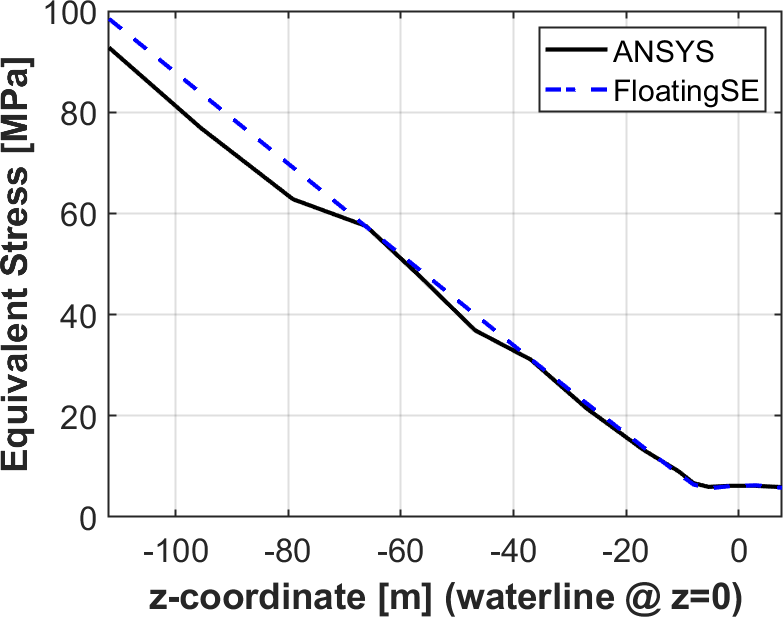
\includegraphics[width=3in]{figs/oc3-verification_equivalentstress.png}
    \caption{Effective (von Mises) stress comparison between
      \textit{FloatingSE} and WISDEM for a pure static loading case.}
    \label{fig:verify}
  \end{center}
\end{figure}

\subsection{With wind and waves}
At this time, more complicated loading cases, with wind and wave loading
included, have not been performed.

\section{Hydrodynamic Verification}
TODO- Check OC3 rigid body modes against projection here

